\chapter{THIẾT KẾ VÀ TRIỂN KHAI HỆ THỐNG}
\begingroup
\clubpenalty=10000
\widowpenalty=10000
\setlength{\parskip}{4pt}
\setlist{itemsep=2pt,parsep=0pt,topsep=3pt}

\section{Yêu cầu thiết kế và lựa chọn linh kiện}
\label{sec:requirements}

\subsection{Yêu cầu của hệ thống}

Từ tên đề tài và điều kiện thực hiện trên kit AVR của học phần, nhóm đặt ra các yêu cầu thiết kế trong Bảng \ref{tab:requirements}. Vi điều khiển ATmega16 có sẵn trên kit nên không thuộc phạm vi lựa chọn; các mục tiếp theo trình bày việc chọn cảm biến và thiết bị hiển thị, cảnh báo.

\begin{table}[H]
\centering
\small
\caption{Yêu cầu thiết kế của hệ thống}
\label{tab:requirements}
\renewcommand{\arraystretch}{1.15}
\begin{tabularx}{\textwidth}{>{\bfseries\raggedright\arraybackslash}p{2.3cm} >{\raggedright\arraybackslash}X >{\raggedright\arraybackslash}p{4.2cm}}
\toprule
Nhóm yêu cầu & Chỉ tiêu & Cách đáp ứng \\
\midrule
Đo nhiệt độ & Nhiệt độ môi trường trong phòng, dải tối thiểu 0--50\,$^\circ$C; cập nhật khoảng 2 giây một lần & DHT11 (mục \ref{sec:sensor-choice}); chu kỳ đọc (mục \ref{sec:threshold}) \\
Hiển thị & Hiện giá trị đo, ngưỡng và thông báo lỗi bằng chữ ngay trên mô hình & LCD 1602 (mục \ref{sec:display-choice}) \\
Cảnh báo & Báo khi nhiệt độ đạt hoặc vượt 30\,$^\circ$C bằng tín hiệu nhìn thấy được; tự trở về khi nhiệt độ giảm & 5 LED trên PD0--PD4 (mục \ref{sec:threshold}) \\
Độ tin cậy & Phát hiện mất tín hiệu và gói tin sai; vi điều khiển không bị treo khi cảm biến hỏng & Timeout và checksum (mục \ref{sec:dht11-read}) \\
Phần cứng & Dùng kit ATmega16 có sẵn, nguồn 5\,V, nạp qua USBasp; hạn chế linh kiện ngoài kit & Kết nối ở Bảng \ref{tab:hardware-wiring} \\
\bottomrule
\end{tabularx}
\end{table}

\subsection{Lựa chọn cảm biến nhiệt độ}
\label{sec:sensor-choice}

Bảng \ref{tab:sensor-compare} so sánh ba cảm biến nhiệt độ phổ biến khi làm việc với vi điều khiển AVR \cite{dht11-datasheet,lm35-datasheet,ds18b20-datasheet}.

\begin{table}[H]
\centering
\small
\caption{So sánh các phương án cảm biến nhiệt độ}
\label{tab:sensor-compare}
\renewcommand{\arraystretch}{1.15}
\setlength{\tabcolsep}{4pt}
\begin{tabularx}{\textwidth}{>{\bfseries\raggedright\arraybackslash}p{2.6cm} >{\raggedright\arraybackslash}X >{\raggedright\arraybackslash}X >{\raggedright\arraybackslash}X}
\toprule
Tiêu chí & LM35 & DS18B20 & DHT11 \\
\midrule
Tín hiệu ra & Điện áp tương tự, 10\,mV/$^\circ$C & Số, bus 1-Wire (Dallas) & Số, Single-Bus (Aosong) \\
Dải đo nhiệt độ & $-55$ đến 150\,$^\circ$C & $-55$ đến 125\,$^\circ$C & 0 đến 50\,$^\circ$C \\
Độ chính xác & 0,5\,$^\circ$C tại 25\,$^\circ$C & $\pm$0,5\,$^\circ$C trong khoảng $-10$ đến 85\,$^\circ$C & $\pm$2\,$^\circ$C \\
Độ phân giải & Phụ thuộc ADC: khoảng 0,49\,$^\circ$C với ADC 10 bit, tham chiếu 5\,V & 0,5 đến 0,0625\,$^\circ$C (9--12 bit) & 1\,$^\circ$C theo tài liệu tham chiếu \\
Nguồn cấp & 4--30\,V & 3,0--5,5\,V & 3,0--5,5\,V \\
Thời gian đọc & Một lần chuyển đổi ADC & Tối đa 750\,ms ở 12 bit & Khoảng 25\,ms; hai lần đọc cách nhau tối thiểu 1\,s \\
Đo độ ẩm & Không & Không & Có (20--90\,\% RH) \\
Kết nối với MCU & Một kênh ADC; dây tín hiệu tương tự dễ nhiễm nhiễu & Một chân GPIO, điện trở kéo lên & Một chân GPIO, điện trở kéo lên \\
\bottomrule
\end{tabularx}
\end{table}

LM35 và DS18B20 chính xác hơn DHT11. Nhóm vẫn chọn DHT11 vì các lý do sau:
\begin{itemize}[leftmargin=1.2cm]
    \item Dải 0--50\,$^\circ$C và sai số $\pm$2\,$^\circ$C đáp ứng yêu cầu cảnh báo ngưỡng 30\,$^\circ$C trong phòng ở Bảng \ref{tab:requirements}.
    \item Tín hiệu số chỉ cần một chân GPIO (PA1); không chiếm kênh ADC và không phụ thuộc điện áp tham chiếu hay nhiễu trên dây như LM35.
    \item Module 3 chân dễ đấu nối ngoài kit; cảm biến đo thêm độ ẩm, cho phép mở rộng chức năng mà không đổi phần cứng.
    \item Giao thức buộc chương trình tự tạo và lấy mẫu xung theo thời gian, phù hợp với nội dung lập trình thanh ghi của học phần.
\end{itemize}
Đổi lại, sai số của DHT11 lớn hơn hai phương án còn lại. Nếu ứng dụng cần độ chính xác cao hơn, DS18B20 có thể thay trên cùng chân PA1, với thay đổi chủ yếu ở phần mềm giao tiếp.

\subsection{Lựa chọn thiết bị hiển thị và cảnh báo}
\label{sec:display-choice}

Kit có sẵn ba thiết bị đầu ra dùng được: LED 7 thanh một chữ số D11, dãy 8 LED đơn trên PORT D và giắc J7 dành cho LCD 1602 (Hình \ref{fig:schematic}). LED 7 thanh một chữ số không đủ để hiện giá trị như \texttt{26.5} hay các thông báo lỗi, đồng thời dùng chung PC0--PC7 với giắc LCD. Nhóm chọn LCD 1602 (2 dòng $\times$ 16 ký tự, bộ điều khiển HD44780) vì đủ chỗ cho giá trị đo, ngưỡng và thông báo chẩn đoán bằng chữ; LCD chạy ở chế độ 4 bit để chỉ chiếm PC4--PC7 và PD5--PD7.

Khối cảnh báo dùng 5 LED đơn trên PD0--PD4: các LED có sẵn trên kit, không cần mạch ngoài và dễ quan sát. Còi báo không có trên kit nên được đưa vào hướng phát triển (mục \ref{sec:future}).

\section{Thiết kế kiến trúc phần cứng và sơ đồ nguyên lý}

\subsection{Sơ đồ khối chức năng và kết nối liên khối hệ thống}

Nhóm vẽ lại sơ đồ giảng viên cung cấp (Hình \ref{fig:schematic}) \cite{hust-kit-manual} và thiết kế PCB trên Altium Designer (Hình \ref{fig:altium-3d}). DHT11 nối ngoài kit theo Hình \ref{fig:system-wiring}. Hệ thống gồm 5 khối chức năng:
\begin{enumerate}[leftmargin=1.2cm, topsep=0pt, itemsep=0.5pt, parsep=0pt]
    \item \textbf{Khối nguồn nuôi 5V}: Cung cấp điện áp +5V ổn định cho toàn mạch qua IC LM7805 hoặc qua cổng USB máy tính.
    \item \textbf{Khối MCU trung tâm}: ATmega16 (DIP-40, dao động nội 8.0 MHz) đảm nhiệm điều phối toàn bộ chu trình hoạt động.
    \item \textbf{Khối cảm biến}: Cảm biến DHT11 thu thập giá trị nhiệt độ và độ ẩm, giao tiếp đơn tuyến với MCU qua chân PA1.
    \item \textbf{Khối hiển thị}: Màn hình LCD 1602 giao tiếp 4-bit qua các chân dữ liệu PC4--PC7 và chân điều khiển PD5--PD7.
    \item \textbf{Khối cảnh báo}: Dàn 5 LED đơn nối với chân PD0--PD4, tích cực mức thấp qua mạng điện trở R4 trên kit.
\end{enumerate}

\begin{figure}[H]\vspace{-0.25cm}
    \centering
    \begin{tikzpicture}[
    font=\small, >=Latex, line width=0.7pt,
    block/.style={draw, rounded corners=3pt, align=center, minimum height=1.5cm, text width=3.6cm, inner sep=6pt, fill=gray!4}
]
\node[block,text width=4.1cm] (power) at (0,0) {\textbf{Nguồn 5V}\\LM7805 (đầu vào 9--12V)\\hoặc 5V từ USBasp};
\node[block,text width=3.3cm,minimum height=2cm] (mcu) at (0,-3.0) {\textbf{ATmega16}\\DIP-40\\RC nội 8 MHz};
\node[block] (dht) at (-5.0,-3.0) {\textbf{Module DHT11 3 chân}\\DATA: PA1\\VCC: 5V; GND chung};
\node[block] (lcd) at (5.0,-1.7) {\textbf{LCD 1602, bus 4-bit}\\D4--D7: PC4--PC7\\RW: PD5; RS: PD6\\EN: PD7};
\node[block] (led) at (5.0,-5.1) {\textbf{5 LED cảnh báo}\\PD0--PD4, Active Low\\Qua mạng điện trở R4};
\draw[->] (power.south) -- node[right]{VCC, GND} (mcu.north);
\draw[<->] (dht.east) -- node[above]{DATA} (mcu.west);
\draw[->] (mcu.east) -- (2.6,-3.0) |- (lcd.west);
\draw[->] (mcu.south) -- (0,-5.1) -- (led.west);
\end{tikzpicture}
\vspace{-0.2cm}
    \caption{Sơ đồ kết nối liên khối chi tiết của hệ thống đo nhiệt độ và cảnh báo}
    \label{fig:system-wiring}
\end{figure}

% Sơ đồ gốc (img/schematic.png) được tách tại khoảng trống dọc giữa khối MCU và
% ba khối bên phải; các khối nối với nhau qua nhãn mạng nên không cắt qua dây nối.
\begin{figure}[p]
    \centering
    \begin{subfigure}{\textwidth}
        \centering
        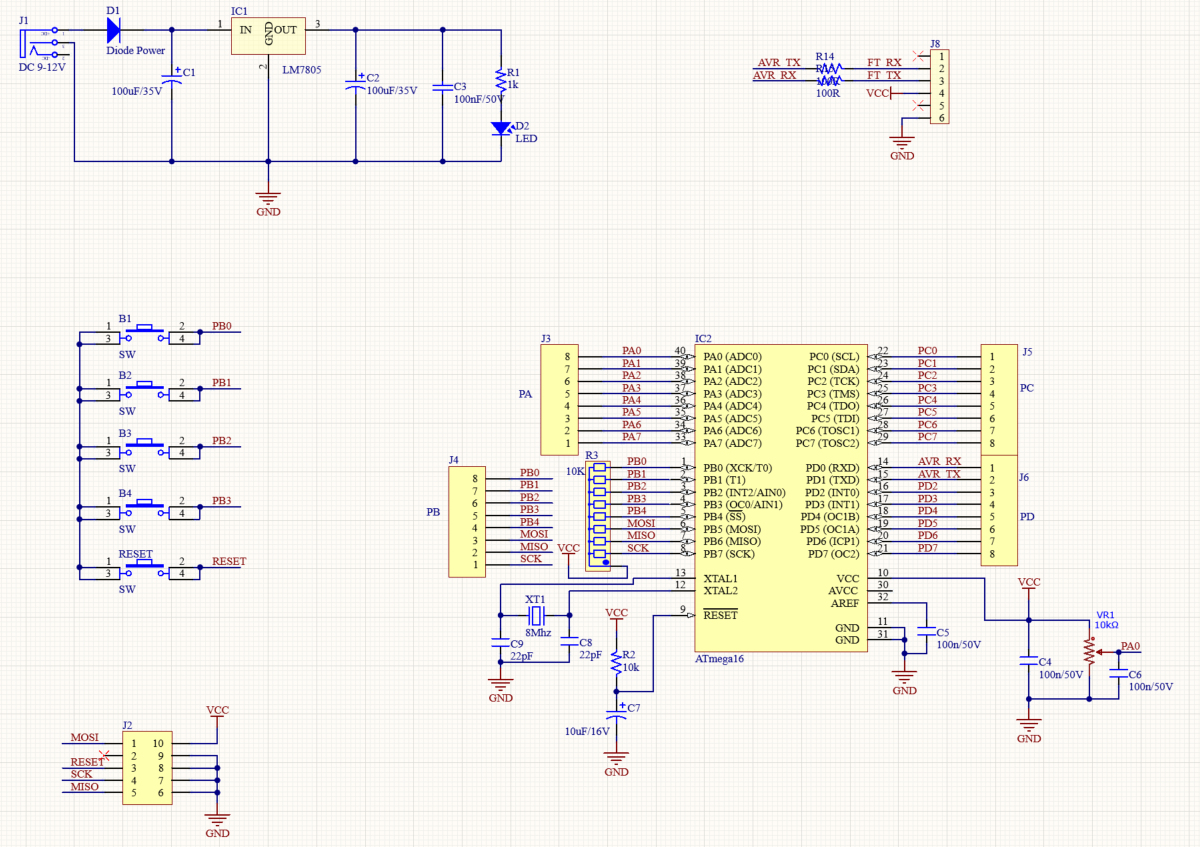
\includegraphics[width=\textwidth]{schematic_main.png}
        \caption{Khối nguồn, vi điều khiển ATmega16, nút bấm, cổng nạp ISP (J2) và các giắc mở rộng cổng}
        \label{fig:schematic-main}
    \end{subfigure}

    \vspace{0.5cm}
    \begin{subfigure}[b]{5.36cm}
        \centering
        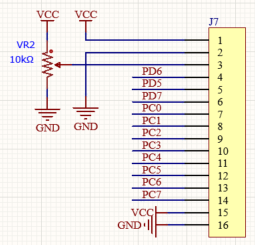
\includegraphics[width=\linewidth]{schematic_lcd.png}
        \caption{Giắc J7 nối LCD 1602}
        \label{fig:schematic-lcd}
    \end{subfigure}\hfill
    \begin{subfigure}[b]{4.31cm}
        \centering
        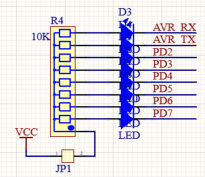
\includegraphics[width=\linewidth]{schematic_led.png}
        \caption{Dãy LED đơn}
        \label{fig:schematic-led}
    \end{subfigure}\hfill
    \begin{subfigure}[b]{5.71cm}
        \centering
        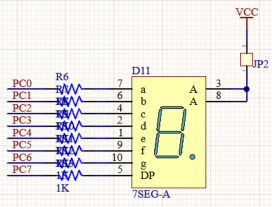
\includegraphics[width=\linewidth]{schematic_7seg.png}
        \caption{LED 7 thanh}
        \label{fig:schematic-7seg}
    \end{subfigure}

    \vspace{0.3cm}
    \caption{Sơ đồ nguyên lý kit AVR được nhóm vẽ lại từ tài liệu giảng viên cung cấp}
    \label{fig:schematic}
    \vspace{0.1cm}
    {\small\textit{Ghi chú:} Các khối (a)--(d) nối với nhau qua nhãn mạng (PA0--PD7, VCC, GND). Trong đồ án, LCD dùng PC4--PC7 và PD5--PD7; 5 LED cảnh báo dùng PD0--PD4. Khối thạch anh XT1 có trên sơ đồ nhưng chương trình chọn dao động RC nội 8 MHz. Cảm biến DHT11 là module nối ngoài, không nằm trong sơ đồ kit này.\par}
\end{figure}

\subsection{Bảng kết nối dây chi tiết giữa các linh kiện}

Bảng \ref{tab:hardware-wiring} liệt kê kết nối giữa từng khối chức năng và chân của ATmega16; số chân tính theo vỏ DIP-40 (Hình \ref{fig:atmega16-pinout}). Tên tín hiệu sau dấu ``/'' là chức năng thay thế của chân, không được dùng trong đồ án.

\begin{table}[tb]
\centering
\small
\caption{Bảng tổng hợp kết nối tín hiệu phần cứng của hệ thống}
\label{tab:hardware-wiring}
\renewcommand{\arraystretch}{1.08}
\setlength{\tabcolsep}{3pt}
\begin{tabularx}{\textwidth}{>{\bfseries\raggedright\arraybackslash}p{2.1cm} >{\raggedright\arraybackslash}p{2.5cm} >{\centering\arraybackslash}p{1.7cm} >{\bfseries\raggedright\arraybackslash}p{2.6cm} >{\raggedright\arraybackslash}X}
\toprule
Khối chức năng & Chân linh kiện & Chân MCU & Tên tín hiệu MCU & Chức năng kỹ thuật \\
\midrule
Cảm biến DHT11 & DATA / S & Chân 39 & PA1 / ADC1 & Giao tiếp Single-Bus hai chiều \\
               & VCC & -- & +5V của kit & Nguồn nuôi +5V DC \\
               & GND & -- & GND của kit & Nối đất chung \\
\midrule
Màn hình LCD   & RS (Chân 4)  & Chân 20 & PD6 / ICP1 & Chọn thanh ghi (0: lệnh, 1: dữ liệu) \\
               & RW (Chân 5)  & Chân 19 & PD5 / OC1A & Chọn đọc/ghi (0: ghi) \\
               & EN (Chân 6)  & Chân 21 & PD7 / OC2 & Xung kích hoạt chốt dữ liệu \\
               & D4 (Chân 11) & Chân 26 & PC4 / TDO & Đường truyền dữ liệu bit 4 \\
               & D5 (Chân 12) & Chân 27 & PC5 / TDI & Đường truyền dữ liệu bit 5 \\
               & D6 (Chân 13) & Chân 28 & PC6 / TOSC1 & Đường truyền dữ liệu bit 6 \\
               & D7 (Chân 14) & Chân 29 & PC7 / TOSC2 & Đường truyền dữ liệu bit 7 \\
\midrule
Dàn LED cảnh báo & Katot LED 1 & Chân 14 & PD0 / RXD & Cảnh báo, sáng khi mức 0 \\
               & Katot LED 2 & Chân 15 & PD1 / TXD & Cảnh báo, sáng khi mức 0 \\
               & Katot LED 3 & Chân 16 & PD2 / INT0 & Cảnh báo, sáng khi mức 0 \\
               & Katot LED 4 & Chân 17 & PD3 / INT1 & Cảnh báo, sáng khi mức 0 \\
               & Katot LED 5 & Chân 18 & PD4 / OC1B & Cảnh báo, sáng khi mức 0 \\
\bottomrule
\end{tabularx}
\end{table}

\begin{figure}[tb]
    \centering
    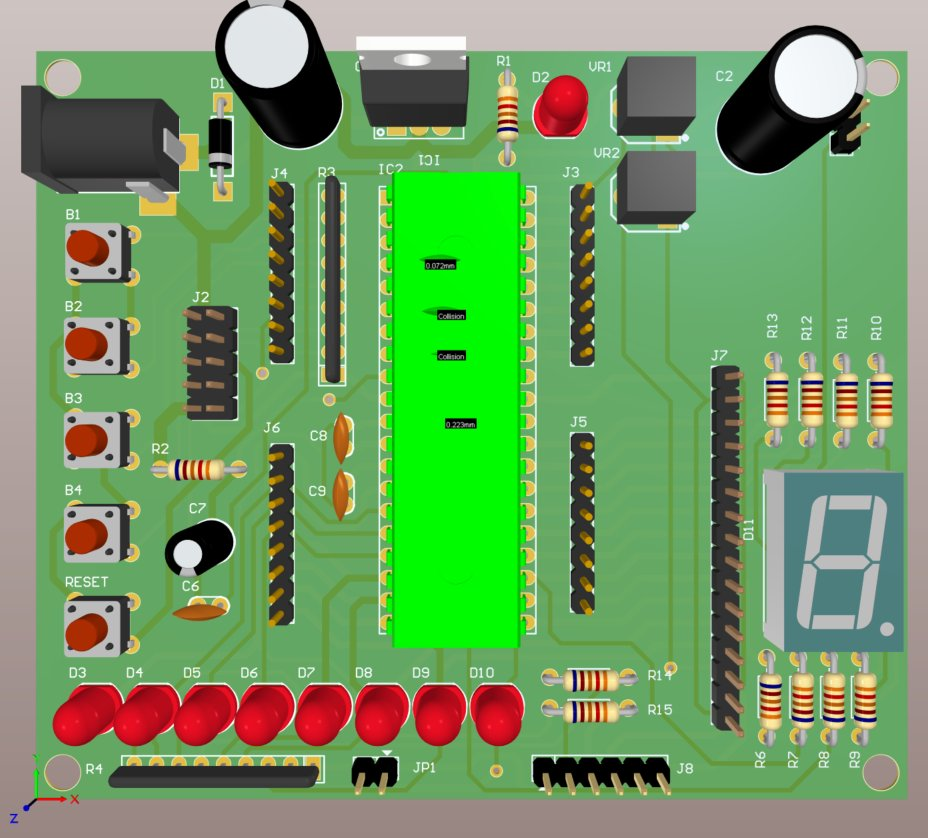
\includegraphics[width=0.48\textwidth]{atmega_kit_3d.png}
    \caption{Mô hình 3D PCB của nhóm trên Altium Designer}
    \label{fig:altium-3d}
\end{figure}

\section{Xây dựng thuật toán và phần mềm điều khiển}

\subsection{Thuật toán điều khiển tổng quát chương trình}
\label{sec:main-algo}

Chương trình vận hành tuần tự theo các bước dưới đây. Lưu đồ ở Hình \ref{fig:main-flowchart} thể hiện cùng các nhánh xử lý; mã nguồn đầy đủ nằm ở Phụ lục A.

\begin{enumerate}[leftmargin=0.8cm,itemsep=6pt,parsep=0pt,topsep=4pt]
    \item \textbf{Khởi tạo hệ thống.} Ghi hai lần bit JTD trong \texttt{MCUCSR} để tắt JTAG và giải phóng PC4, PC5. Khởi tạo LCD bằng \texttt{LCD4\_INIT}; đặt PD0--PD4 làm đầu ra (\texttt{DDRD |= 0x1F}) và xuất mức cao để tắt LED (\texttt{PORTD |= 0x1F}). LCD hiện \texttt{DA2: DO NHIET DO} và \texttt{DHT11 SENSOR} khoảng 1,5 giây, sau đó được xóa.
    \item \textbf{Đọc cảm biến.} Gọi \texttt{DHT11\_Read} để nhận dữ liệu nhiệt độ cùng mã trả về \texttt{status}. Chương trình chỉ so sánh ngưỡng và hiển thị nhiệt độ khi \texttt{status == 0}.
    \item \textbf{Xử lý dữ liệu hợp lệ.} Dòng 1 LCD hiển thị nhiệt độ theo định dạng \texttt{Temp: XX.Y °C}. Dòng 2 hiển thị ngưỡng; các khoảng trắng cuối chuỗi được dùng để ghi đè nội dung cũ trong 16 vị trí:
    \begin{itemize}[leftmargin=0.6cm,itemsep=3pt,topsep=3pt]
        \item Nếu \texttt{temp\_int >= 30}: hiện \texttt{HIGH Th: 30°C *!}; dùng \texttt{PORTD \&= 0xE0} kéo PD0--PD4 xuống mức thấp, bật 5 LED.
        \item Nếu \texttt{temp\_int < 30}: hiện \texttt{HIGH Th: 30°C}, xóa dấu \texttt{*!}; dùng \texttt{PORTD |= 0x1F} tắt 5 LED.
    \end{itemize}
    \item \textbf{Xử lý lỗi.} Không dùng lại dữ liệu cũ để so sánh ngưỡng. Cả hai nhánh lỗi đều tắt 5 LED bằng \texttt{PORTD |= 0x1F}:
    \begin{itemize}[leftmargin=0.6cm,itemsep=3pt,topsep=3pt]
        \item \texttt{status == -6}: hiện \texttt{DHT11: Sum Error} và \texttt{Checksum Invalid} trên hai dòng LCD.
        \item \texttt{status} từ -1 đến -5: hiện \texttt{DHT11: No Signal} và \texttt{Check Pin PA1}, tương ứng với timeout khi chờ tín hiệu.
    \end{itemize}
    Việc tắt LED khi lỗi tránh cảnh báo dựa trên dữ liệu cũ, nhưng cũng làm hệ thống không cảnh báo được nếu môi trường đang quá nhiệt; hạn chế này được nêu ở mục \ref{sec:conclusion-limits}.
    \item \textbf{Lặp lại.} Thực hiện \texttt{\_delay\_ms(2000)}, rồi quay lại bước đọc cảm biến. Thời gian giữa hai lượt đọc còn bao gồm giao tiếp và cập nhật LCD, như phân tích ở mục \ref{sec:threshold}.
\end{enumerate}

\begin{figure}[p]
\centering
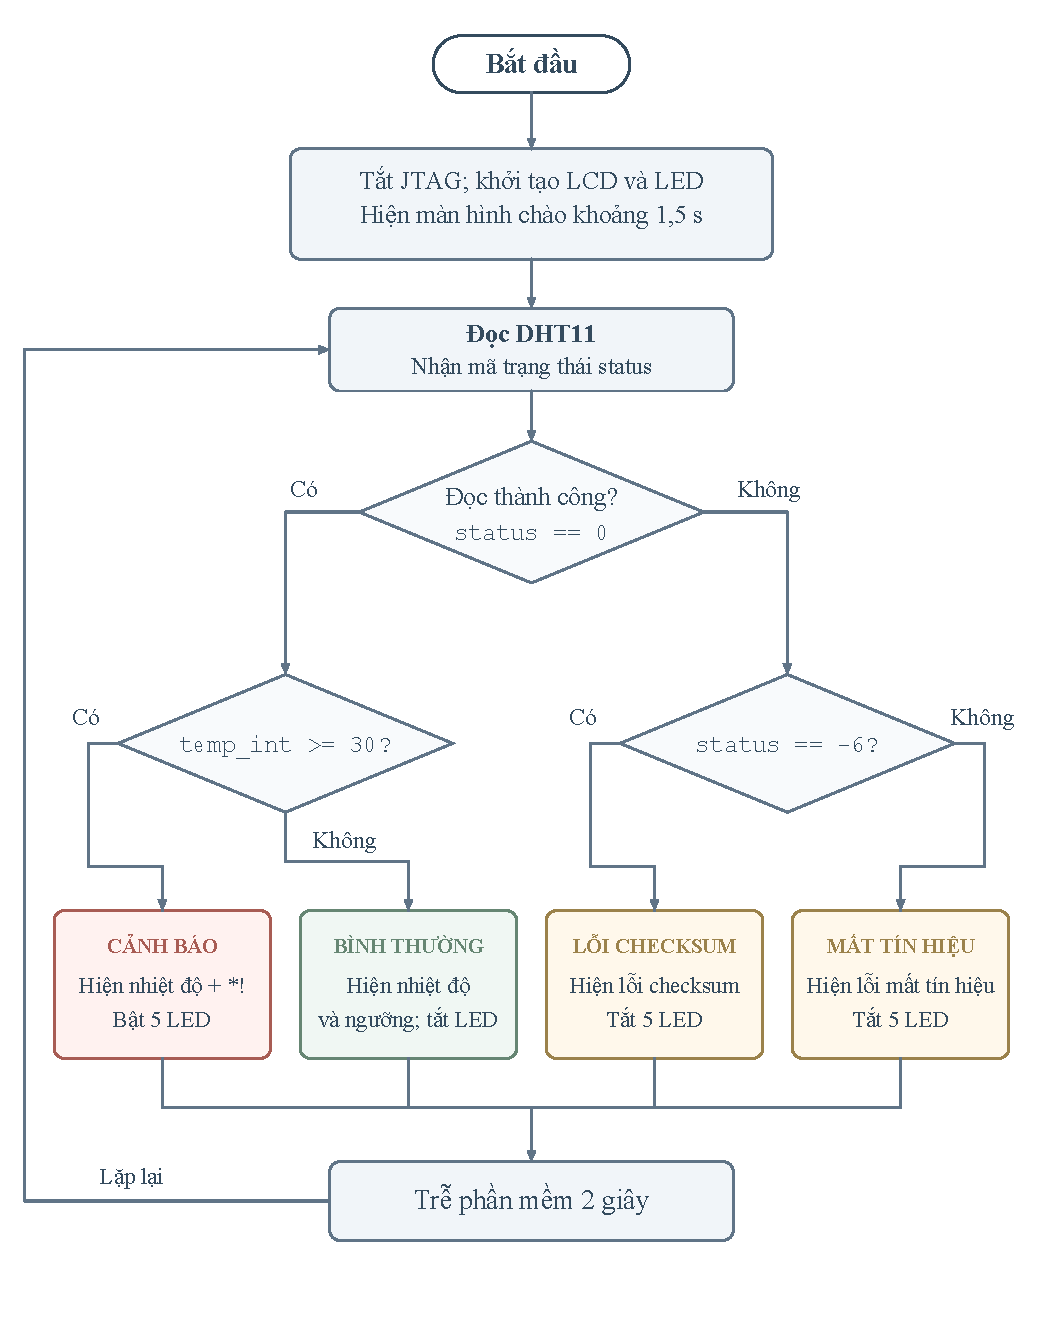
\includegraphics[width=\textwidth,height=0.88\textheight,keepaspectratio]{diagrams/main-flowchart.pdf}
\caption{Lưu đồ thuật toán đo nhiệt độ, cảnh báo và xử lý lỗi}
\label{fig:main-flowchart}
\end{figure}

\subsection{Thuật toán giao tiếp và giải mã cảm biến DHT11}
\label{sec:dht11-read}

Hàm \texttt{DHT11\_Read(uint8\_t *temp\_int, uint8\_t *temp\_dec, uint8\_t *humi\_int)} được viết trực tiếp bằng thao tác thanh ghi để tạo và lấy mẫu xung theo các mốc thời gian của giao thức, kèm cơ chế timeout chống treo vi điều khiển.

\subsubsection{Cơ chế chống treo bằng timeout}
Nếu chân DATA bị hở mạch hoặc cảm biến hỏng, các vòng chờ sườn xung như \texttt{while(DHT\_PIN\_R \& (1 << DHT\_BIT))} sẽ lặp vô hạn và vi điều khiển bị treo. Vì vậy mỗi vòng chờ được gắn một biến đếm giảm dần \texttt{timeout = 10000}; khi biến đếm về 0 mà trạng thái chân chưa đổi, hàm thoát và trả về mã lỗi âm ứng với vòng chờ đó.

Thời gian timeout được xác định từ mã máy do \texttt{avr-gcc} sinh ra với tùy chọn \texttt{-Os} (xem bằng \texttt{avr-objdump -d}). Mỗi lần lặp của bốn vòng chờ đầu gồm lệnh kiểm tra bit \texttt{sbic}/\texttt{sbis} (1 chu kỳ), \texttt{rjmp} (2), \texttt{sbiw} (2) và \texttt{brne} (2), tổng cộng 7 chu kỳ. Ở vòng chờ thứ năm, lệnh \texttt{sbis} nhảy qua \texttt{rjmp} (2 chu kỳ) nên mỗi lần lặp tốn 6 chu kỳ. Kết quả ở 8\,MHz được tổng hợp trong Bảng \ref{tab:timeout}.

\begin{table}[H]
\centering
\small
\caption{Thời gian timeout của các vòng chờ trong \texttt{DHT11\_Read} ở 8 MHz}
\label{tab:timeout}
\renewcommand{\arraystretch}{1.15}
\begin{tabularx}{\textwidth}{c X c c}
\toprule
\textbf{Mã lỗi} & \textbf{Vòng chờ} & \textbf{Chu kỳ/lần lặp} & \textbf{Timeout} \\
\midrule
$-1$ & DHT11 kéo đường DATA xuống mức thấp sau xung khởi động & 7 & 8,75\,ms \\
$-2$ & DHT11 kéo đường DATA lên mức cao (tín hiệu phản hồi) & 7 & 8,75\,ms \\
$-3$ & DHT11 kéo đường DATA xuống mức thấp trước bit đầu tiên & 7 & 8,75\,ms \\
$-4$ & Kết thúc mức thấp 50\,$\mu$s ở đầu mỗi bit & 7 & 8,75\,ms \\
$-5$ & Kết thúc mức cao của bit `1' & 6 & 7,5\,ms \\
\bottomrule
\end{tabularx}
\end{table}

Khi rút dây DATA, điện trở kéo lên giữ PA1 ở mức cao, vòng chờ đầu tiên hết hạn và hàm trả về $-1$ sau khoảng 20\,ms (xung khởi động) + 8,75\,ms $\approx$ 29\,ms, không đáng kể so với chu kỳ 2 giây. Các giá trị trên tỷ lệ nghịch với tần số thực của dao động RC nội. Cũng từ mã máy, \texttt{\_delay\_us(38)} được biên dịch thành vòng trễ 304 chu kỳ, đúng 38\,$\mu$s ở 8\,MHz.

\subsubsection{Giải mã bit dữ liệu}
Bit `0' có mức cao kéo dài 26--28\,$\mu$s, bit `1' khoảng 70\,$\mu$s (mục \ref{sec:dht11-protocol}). Thời điểm lấy mẫu 38\,$\mu$s nằm giữa hai giá trị này: nếu PA1 còn ở mức cao thì bit là `1', nếu đã về mức thấp thì bit là `0'. Sau xung khởi động và tín hiệu phản hồi, vòng lặp lồng nhau quét 5 byte (40 bit); mỗi bit được giải mã theo các bước:
\begin{enumerate}[leftmargin=1.2cm]
    \item Đợi kết thúc xung mức LOW 50 $\mu$s của bit đang truyền.
    \item Đưa CPU vào trạng thái trễ 38 $\mu$s (\texttt{\_delay\_us(38)}).
    \item Đọc thanh ghi \texttt{PINA}: nếu bit PA1 đang ở mức 1, ta ghi nhận đây là bit '1' bằng phép dịch bit:
    \begin{samepage}
\begin{verbatim}
    data[i] |= (1 << j);
    \end{verbatim}
\par\end{samepage}
    Tiếp tục chờ xung mức HIGH kết thúc trước khi đón nhận bit tiếp theo.
\end{enumerate}

\subsubsection{Kiểm tra checksum và mã trả về}
Cuối hàm \texttt{DHT11\_Read}, tổng của 4 byte đầu được so sánh với byte thứ 5 (byte checksum):
\begin{verbatim}
if ((uint8_t)(data[0] + data[1] + data[2] + data[3]) != data[4]) {
    return -6; // Lỗi sai Checksum
}
\end{verbatim}
Nếu khớp, các con trỏ nhận giá trị tương ứng và hàm trả về 0. Như vậy hàm có ba nhóm mã trả về: 0 khi đọc thành công; $-1$ đến $-5$ khi hết thời gian ở một trong năm vòng chờ của Bảng \ref{tab:timeout}; $-6$ khi sai checksum. Cách \texttt{main()} xử lý từng nhóm mã được trình bày ở bước 4 của mục \ref{sec:main-algo}.

\subsection{Xây dựng thư viện điều khiển màn hình LCD 1602}

Thư viện \texttt{hunget\_lcd.h} được xây dựng với sự hỗ trợ của công cụ sinh mã và cấu hình cho cách nối chân của kit. Các hàm dưới đây trình bày nguyên lý truyền dữ liệu, tạo xung Enable và giữ nguyên các bit không dùng cho LCD; việc dùng công cụ hỗ trợ không thay thế bước kiểm tra trên phần cứng.

\subsubsection{Hàm tạo xung chốt dữ liệu (\texttt{LCD\_Enable})}
Theo chuẩn Hitachi HD44780, dữ liệu tại bus 4-bit chỉ được bộ điều khiển LCD ghi nhận tại thời điểm sườn xuống của chân Enable (chân PD7). Do vi điều khiển chạy ở tần số 8.0 MHz (mỗi chu kỳ clock dài $0.125\text{ }\mu\text{s}$), hàm tạo xung cần bảo đảm thời gian thiết lập và thời gian giữ dữ liệu:
\begin{verbatim}
static inline void LCD_Enable(void) {
    LCD_CTRL_PORT |= (1 << LCD_EN);
    _delay_us(5);
    LCD_CTRL_PORT &= ~(1 << LCD_EN);
    _delay_us(100);
}
\end{verbatim}

\subsubsection{Hàm truyền 4 bit dữ liệu (\texttt{LCD\_Send4Bit})}
Do cổng PORT C chỉ dùng 4 chân cao (PC4 -- PC7) cho LCD, việc ghi dữ liệu ra LCD không được làm thay đổi trạng thái của 4 chân thấp (PC0 -- PC3). Do đó chương trình dùng phép AND/OR với mặt nạ bit:
\begin{verbatim}
static inline void LCD_Send4Bit(unsigned char Data) {
    unsigned char current_port_c = LCD_DATA_PORT & 0x0F;
    LCD_DATA_PORT = current_port_c | (Data & 0xF0);
    LCD_Enable();
}
\end{verbatim}

\subsubsection{Trình tự khởi tạo chế độ 4-bit (\texttt{LCD4\_INIT})}
Khi mới cấp điện, màn hình LCD có thể chưa ở trạng thái giao tiếp mong muốn. Trình tự khởi tạo phần mềm bằng chuỗi lệnh gửi 3 lần mã \texttt{0x30} cách nhau các khoảng trễ hợp lý giúp đưa vi mạch HD44780 về trạng thái reset đồng bộ, sau đó chuyển sang chế độ 4-bit bus (\texttt{0x20}) và cấu hình hiển thị 2 dòng ma trận $5 \times 8$ (\texttt{0x28}).

\subsection{Thuật toán so sánh ngưỡng cảnh báo và điều khiển LED}
\label{sec:threshold}

Ngưỡng nhiệt độ cảnh báo của hệ thống được cố định tại giá trị $30^\circ\text{C}$ (\texttt{HIGH Th: 30°C}). Đây là mốc kiểm thử để quan sát sự chuyển trạng thái của mô hình trong điều kiện phòng và gia nhiệt nhẹ, không phải ngưỡng an toàn được suy ra từ yêu cầu của một ứng dụng cụ thể. Với dữ liệu nhiệt độ không âm theo định dạng đang dùng, phép so sánh \texttt{temp\_int >= 30} cũng kích hoạt cảnh báo tại đúng $30^\circ\text{C}$.

Hệ thống chưa có vùng trễ (hysteresis): cùng một ngưỡng được dùng để bật và tắt cảnh báo. Nếu số đo dao động quanh $30^\circ\text{C}$, LED có thể đổi trạng thái qua các lần đọc. Đây là hạn chế cần khảo sát ở các điểm sát ngưỡng.

Khi điều khiển dàn LED trên PORT D, thách thức kỹ thuật đặt ra là các chân PD5, PD6, PD7 đang đảm nhiệm điều khiển các chân tín hiệu RW, RS, EN của màn hình LCD. Nếu ghi trực tiếp một giá trị vào thanh ghi \texttt{PORTD}, các tín hiệu điều khiển LCD sẽ bị ghi đè và LCD có thể nhận sai lệnh hoặc dữ liệu.

Để giải quyết bài toán dùng chung cổng ngoại vi này, chương trình dùng mặt nạ bit:
\begin{itemize}[leftmargin=1.2cm]
    \item Khi nhiệt độ vượt ngưỡng ($temp\_int \ge 30^\circ\text{C}$): Cần đưa 5 bit thấp (PD0 -- PD4) về mức 0 (bật sáng LED), nhưng giữ nguyên giá trị của 3 bit cao (PD5 -- PD7). Phép toán \texttt{AND} với mặt nạ \texttt{0xE0} (nhị phân \texttt{1110 0000}) được sử dụng:
    \begin{equation}
        \text{PORTD} = \text{PORTD} \ \& \ \text{0xE0}
    \end{equation}
    \item Khi giá trị nhiệt độ dưới ngưỡng ($temp\_int < 30^\circ\text{C}$): Cần đưa 5 bit thấp (PD0 -- PD4) lên mức 1 (tắt LED), đồng thời bảo toàn 3 bit cao (PD5 -- PD7). Phép toán \texttt{OR} với mặt nạ \texttt{0x1F} (nhị phân \texttt{0001 1111}) được sử dụng:
    \begin{equation}
        \text{PORTD} = \text{PORTD} \ | \ \text{0x1F}
    \end{equation}
\end{itemize}

Nhờ kỹ thuật che mặt nạ bit này, khối cảnh báo LED và khối hiển thị LCD cập nhật các nhóm chân riêng biệt trên cùng một cổng PORT D. Chuỗi cảnh báo hiển thị trên dòng 2 của màn hình LCD có định dạng \texttt{"HIGH Th: 30°C *!"} với đúng 16 ký tự, vừa đủ 16 vị trí hiển thị của một dòng LCD 1602. Sau mỗi vòng lặp, chương trình thực hiện \texttt{\_delay\_ms(2000)}. Chu kỳ giữa hai lần bắt đầu đọc liên tiếp còn bao gồm thời gian giao tiếp DHT11 và cập nhật LCD:
\begin{equation}
T_{\text{chu kỳ}} \approx 2.0\,\text{s} + T_{\text{đọc}} + T_{\text{LCD}} + T_{\text{xử lý}}.
\end{equation}
Do đó chu kỳ thực tế lớn hơn 2 giây ở tần số danh định, không phải bộ định thời lấy mẫu chính xác 2 giây. Các khoảng trễ phụ thuộc tần số RC nội thực tế và cấu hình \texttt{F\_CPU} \cite{avrgcc-manual}.

\section{Quy trình biên dịch và nạp firmware}

\subsection{Quy trình tự động hóa với Makefile}

Mã nguồn dự án được tổ chức và biên dịch tự động hóa thông qua công cụ GNU Make và bộ biên dịch \texttt{avr-gcc} \cite{avrgcc-manual}. Tập tin \texttt{Makefile} thiết lập các quy tắc dịch mã:
\begin{itemize}[leftmargin=1.2cm]
    \item Thiết lập cờ biên dịch: \texttt{-Wall -Os -mmcu=atmega16} \texttt{-DF\_CPU=8000000UL} (tối ưu mã máy \texttt{-Os}, tần số 8~MHz).
    \item Quy tắc tạo file \texttt{tempsen.elf} từ file nguồn \texttt{tempsen.c} và file tiêu đề \texttt{hunget\_lcd.h}.
    \item Quy tắc chuyển đổi định dạng \texttt{tempsen.hex}: Sử dụng công cụ \texttt{avr-objcopy -O ihex -R .eeprom tempsen.elf tempsen.hex} để tạo file mã máy tiêu chuẩn Intel HEX sẵn sàng nạp vào bộ nhớ Flash ROM.
    \item Lệnh \texttt{avr-size tempsen.elf} báo dung lượng bộ nhớ mà chương trình sử dụng; kết quả ở Bảng \ref{tab:memory}.
\end{itemize}

Cấu hình nạp fuse trong Makefile dùng \texttt{LFUSE = 0xE4} và \texttt{HFUSE = 0xD9}, thống nhất với nguồn clock RC nội 8 MHz trong báo cáo. Lệnh \texttt{make fuse} ghi các giá trị này; việc biên dịch với \texttt{F\_CPU} không tự thay đổi fuse phần cứng.

\begin{table}[H]
\centering
\small
\caption{Dung lượng bộ nhớ của chương trình (\texttt{avr-size}, avr-gcc 16.1.0, \texttt{-Os})}
\label{tab:memory}
\renewcommand{\arraystretch}{1.15}
\begin{tabularx}{\textwidth}{>{\bfseries}l X r r r}
\toprule
Vùng nhớ & Thành phần & Sử dụng & Dung lượng chip & Tỷ lệ \\
\midrule
Flash & \texttt{.text} (2674 B) + \texttt{.data} (156 B) & 2830 B & 16384 B & 17,3\,\% \\
SRAM & \texttt{.data} (156 B) + \texttt{.bss} (0 B), chưa tính ngăn xếp & 156 B & 1024 B & 15,2\,\% \\
EEPROM & Không sử dụng & 0 B & 512 B & 0\,\% \\
\bottomrule
\end{tabularx}
\end{table}

Toàn bộ 156 B của vùng \texttt{.data} là các chuỗi hằng hiển thị trên LCD (cùng chuỗi định dạng \texttt{"\%05u"} của thư viện LCD); chúng được chép từ Flash sang SRAM khi khởi động. Biến cục bộ như \texttt{buffer[32]} trong \texttt{main()} và vùng nhớ tạm của \texttt{sprintf} nằm trên ngăn xếp nên không có trong số liệu này. Chương trình còn nhiều dư địa bộ nhớ cho các hướng mở rộng ở mục \ref{sec:future}.

\subsection{Quy trình nạp chương trình bằng phần mềm ProgISP}
\label{sec:progisp}

Các bước nạp chương trình vào ATmega16 được trình bày dưới đây; giao diện tham khảo ở Hình \ref{fig:progisp-setup}.

\begin{enumerate}[leftmargin=1.2cm]
    \item Kết nối USBasp giữa máy tính và cổng ISP trên kit.
    \item Mở ProgISP 1.72.
    \item Tại \textit{Select Chip}, chọn \texttt{ATMEGA16}.
    \item Nhấn RD (Read) để kiểm tra kết nối; mã nhận diện dự kiến là \texttt{1E : 94 : 03}.
    \item Đặt High Fuse = \texttt{0xD9}, Low Fuse = \texttt{0xE4} (mã \texttt{0xD9E4}); bật tùy chọn \textit{Program Fuse}.
    \item Nhấn \textit{Load Flash}, chọn tệp \texttt{src/tempsen.hex}.
    \item Nhấn \textit{Auto} để xóa chip, ghi và kiểm tra Flash, ghi fuse. Khi báo \textit{Successfully done}, vi điều khiển khởi động lại và chạy chương trình.
\end{enumerate}

\begin{figure}[H]
\centering
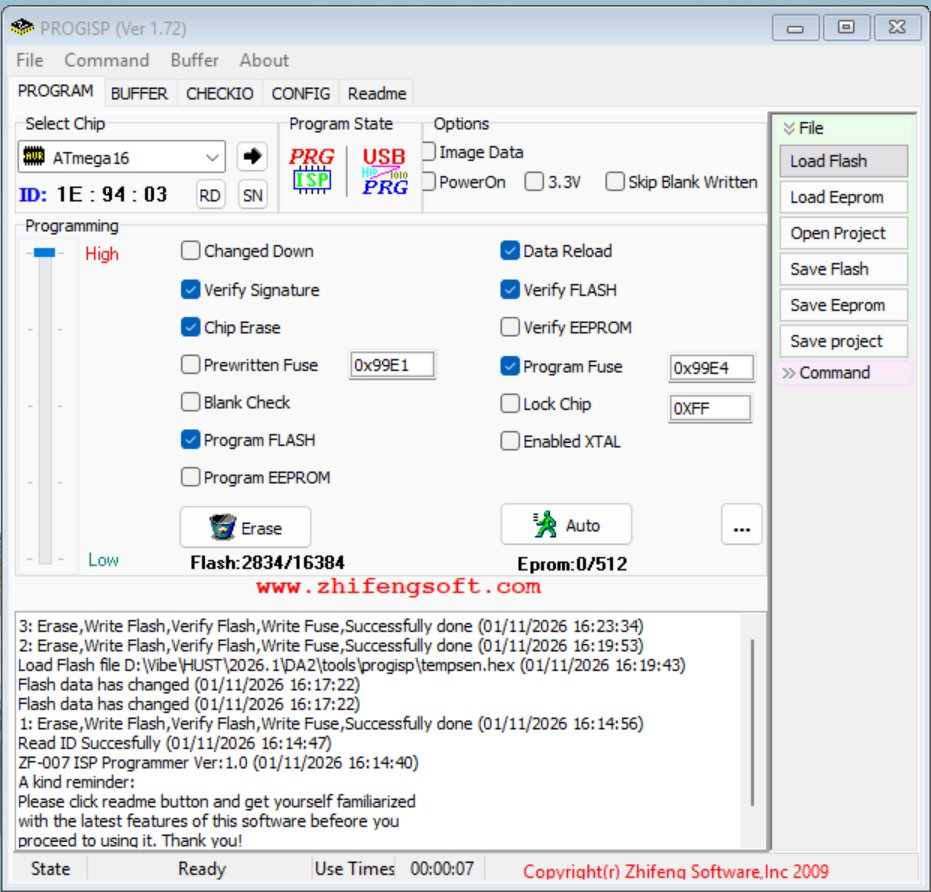
\includegraphics[width=0.72\textwidth,keepaspectratio]{progisp_setup.png}
\caption{Giao diện ProgISP khi nạp firmware và cấu hình fuse \texttt{0xD9E4}}
\label{fig:progisp-setup}
\end{figure}

\endgroup
